This project will be developed in a web environment to ensure the creation of a platform independent system. It will primarily use Three.js~\footnote{\bibentry{cabello2010three}}, a JavaScript library that abstracts WebGL, as a tool for creating 3D visualisations. An initial prototype was designed and has been discussed in Appendix~\ref{app:current_progress}. The main \emph{goals} of this project are to:

\begin{itemize}
	\item Visualise a large dataset in a time efficient manner.
	% \item Ensure the visualisation is aesthetically pleasing and useful to the user.
	% 	\begin{itemize}
	% 		\item Users should be able to understand and interpret the data without training.
	% 	\end{itemize}
	\item Create visualisations that can be applied to multiple datasets.
	\item Integrate the results into the teaching analytics component of the group project.
	\item Explore how 3D visualisations can effectively convey information.
	\item Apply the visualisations to real datasets and ensure they are scalable.
	\item Explore how to optimise calls and understand what drains processing resources easily.
	\begin{itemize}
		\item This can be measured with a JavaScript performance testing environment~\footnote{\bibentry{bynens2011jsperf}}.
	\end{itemize}
\end{itemize}

To facilitate these goals, this project will involve creating visualisations that can be: applied to a range of datasets and compared to one another. This will require applying the same datasets to both visualisations and analysing the differences in performance and scalability. With this in mind, it has been decided that heat maps will be used as the basis of this project as they have a wide array of applications. Figure~\ref{fig:heat_maps} features two different ways of visualising a heat map. It has potential applications in displaying a 3D column or bar chart, financial and geographical data. It is interesting to note that geographical data can be applied to both visualisations, where the image on the left can be mapped to a sphere and could represent population data, while the other could represent pollution levels in a city.

\newcommand{\heatmapwidth}{0.4\textwidth}
\newcommand{\heatmapheight}{3.5cm}
\begin{figure}[H]
	\centering
	\begin{subfigure}[b]{\heatmapwidth}
        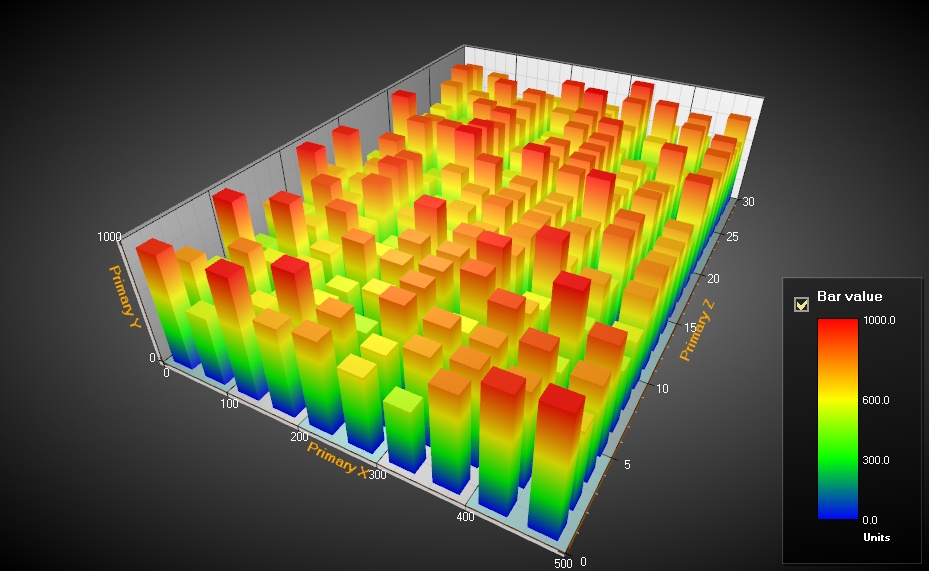
\includegraphics[width=\textwidth,height=\heatmapheight]{images/heat-map-1}
        \caption{A heat map of financial data. \protect\footnotemark}
        \label{fig:heat_map_financial}
    \end{subfigure}
    \begin{subfigure}[b]{\heatmapwidth}
        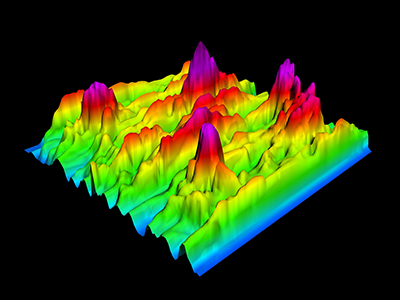
\includegraphics[width=\textwidth,height=\heatmapheight]{images/heat-map-2}
        \caption{A heat map of electroencephalogram. \protect\footnotemark}
        \label{fig:heat_map_eeg}
    \end{subfigure}
	\caption{Two different representations of a heat map.}
	\subfigcaptionskip
	\label{fig:heat_maps}
\end{figure}

\addtocounter{footnote}{-2}
	\stepcounter{footnote}\footnotetext{\bibentry{tuomainen2014financial}}
	\stepcounter{footnote}\footnotetext{\bibentry{fuchs2006physiological}}

The data for the visualisations can easily be represented as a flat array and may need to be preprocessed, which depends on the format of the data. This data representation has also been adopted by The WebGL Globe Chrome Experiment~\footnote{\bibentry{google2011globe}}, as shown in Appendix~\ref{app:globe}, is a great example of visualising a large dataset in an efficient way. This open platform project clearly demonstrates that the goals of this project are achievable. They encourage users to use their own datasets, ensuring a certain level of scalability and applications with geographical data.

The development of these visualisations will involve using the established \href{http://threejs.org/docs/#Reference/Extras.Geometries/BoxGeometry}{BoxGeometry} and NURBS surface that are available in Three.js. The \href{http://threejs.org/examples/webgl_geometry_nurbs.html}{NURBS example}, as displayed in Appendix~\ref{app:nurbs}, proves that it is possible to render a smooth 3D surface. This can be applied to represent a heat map and if there lie difficulties in implementing this, then a simpler representation can be modelled.

\section{Deliverables} {
\label{sec:deliverables}

	The key deliverables of this project have been split into three categories: basic, intermediate and advanced.

	The \emph{basic deliverables} entail developing the implementation for a single visualisation, which should resemble Figure~\ref{fig:heat_map_financial}, with a small, generated dataset. This visualisation will have interactions for panning, zooming and rotating enabling users to navigate the scene.

	The \emph{intermediate deliverables} are concerned with providing users with the ability to filter data, so they are able hide particular information shown on the visualisation. This set of deliverables will also see the implementation of another visualisation, similar to Figure~\ref{fig:heat_map_eeg}, which will initially be applied to a large, generated dataset. The final stage of these deliverables involves applying real datasets, as outlined in Section~\ref{sec:dataset}, to both visualisations.

	The core \emph{advanced deliverables} requires integrating both prototypal visualisations into the group project. Other deliverables include analysing the scalability and computational power to render both visualisations, performing a user study to measure the usefulness of the visualisations and incorporating multi-touch gestures such as pan, pinch, zoom and rotate.

}

\section{Dataset} {
\label{sec:dataset}

	As discussed in Section~\ref{sec:deliverables}, the visualisations will begin with generated data so development can begin immediately. Using generated data brings control over the size of the dataset applied to a prototype and enables the scalability of each visualisation can be tested. 

	Following the use of fake data, each prototype will have real datasets applied to them. By using the same data for both prototypes, their differences in computational requirements and scalability can be compared and analysed. GeoNames~\footnote{\bibentry{wick2005geonames}} is a geographical database that stores population data for a significant number of cities and their respective latitude and longitude coordinates. This database falls under a creative commons attribution license and will be used for both visualisations because there are no copyright concerns or immediate issues when reading and parsing the data it provides. However, some unnecessary information contained in a GeoNames dataset (such as \emph{geonameid}, \emph{feature class} and  \emph{dem}) will need to be removed. The format of the data should also be modified (from a tab separated list to a JavaScript array) when used with a prototype. These steps are necessary so the visualisations can read the data efficiently and hence reduce the loading time for the user. Other datasets can be obtained from Earthdata~\footnote{\bibentry{nasa2000data}}, but will require further investigation regarding how to extract the information from the available databases.

	Once real data has been applied to both prototypes, the visualisations will be integrated into a live system for the teaching analytics component of the final year project. The amount of touch gestures that particular system components receive and the progress made by students, groups and tutorials will need to be collected and stored in the database. This data can be visualised to aid teachers in analysing ongoing student progress.

}

\section{Evaluation} {
\label{sec:evaluation}

	The following criteria will be considered when evaluating and comparing the visualisations: time to render, time to perform operations after render, average frames per second, scaling betwen small and large datasets and how different colours and schemes effect performance.

}

\section{Methodology} {
\label{sec:methodology}

	A rapid application development (RAD) approach will be undertaken when developing this project. This methodology focuses on iterative development and the rapid construction of prototypes, instead of investing significant amounts of time into planning. RAD enables the software to be written quickly through the reuse of software components and engaging in less formal reviews. This process also performs unit, integration and system testing at the end of each construction phase. 

	In this project, each visualisation can be thought of as a single prototype, where parts of the first prototype can be reused for the second visualisation. Testing should be performed during the course of the project, but particularly when a major component of a prototype has been developed, such as data filtering.

}

\section{Non-functional requirements} {

	The following non-functional requirements are considered key to the success of this project:

	\begin{description}
		\item[Modularity:] The project should be highly modular, so parts of the system can be reused and easily integrated into the group project.
		\item[Performance:] The response time of the system is a major concern when working with a large dataset. The time to load the visualisation is highly dependent on the size of the dataset, graphical processing, network bandwidth and latency. However, once the visualisation has loaded, the user should be faced with near immediate response times (\textless 1 second).
		\item[Scalability:] This is important when modifying the size of the dataset used with a visualisation. The visualisation should be capable of handling increased processing with a larger dataset. Not only this, but the information should remain mapped to the correct locations in the scene with increased volumes of data.
		\item[Testability:] Highly testable code is important when writing test suites, so all aspects of the system can be easily tested to locate faults. In JavaScript:
			\begin{itemize}
				\item A common technique is to hide variables through the use of closure, which leads to untestable code. These variables should be replaced with public variables that are prefixed with an underscore, to indicate they are not a part of the public API.
				\item Anonymous functions should be replaced with named functions so they can be tested.
				\item Dependency injection should be used through RequireJS, so all dependencies can be mocked.
			\end{itemize}
	\end{description}

}
